\documentclass[1p]{elsarticle_modified}
%\bibliographystyle{elsarticle-num}

%\usepackage[colorlinks]{hyperref}
%\usepackage{abbrmath_seonhwa} %\Abb, \Ascr, \Acal ,\Abf, \Afrak
\usepackage{amsfonts}
\usepackage{amssymb}
\usepackage{amsmath}
\usepackage{amsthm}
\usepackage{scalefnt}
\usepackage{amsbsy}
\usepackage{kotex}
\usepackage{caption}
\usepackage{subfig}
\usepackage{color}
\usepackage{graphicx}
\usepackage{xcolor} %% white, black, red, green, blue, cyan, magenta, yellow
\usepackage{float}
\usepackage{setspace}
\usepackage{hyperref}

\usepackage{tikz}
\usetikzlibrary{arrows}

\usepackage{multirow}
\usepackage{array} % fixed length table
\usepackage{hhline}

%%%%%%%%%%%%%%%%%%%%%
\makeatletter
\renewcommand*\env@matrix[1][\arraystretch]{%
	\edef\arraystretch{#1}%
	\hskip -\arraycolsep
	\let\@ifnextchar\new@ifnextchar
	\array{*\c@MaxMatrixCols c}}
\makeatother %https://tex.stackexchange.com/questions/14071/how-can-i-increase-the-line-spacing-in-a-matrix
%%%%%%%%%%%%%%%

\usepackage[normalem]{ulem}

\newcommand{\msout}[1]{\ifmmode\text{\sout{\ensuremath{#1}}}\else\sout{#1}\fi}
%SOURCE: \msout is \stkout macro in https://tex.stackexchange.com/questions/20609/strikeout-in-math-mode

\newcommand{\cancel}[1]{
	\ifmmode
	{\color{red}\msout{#1}}
	\else
	{\color{red}\sout{#1}}
	\fi
}

\newcommand{\add}[1]{
	{\color{blue}\uwave{#1}}
}

\newcommand{\replace}[2]{
	\ifmmode
	{\color{red}\msout{#1}}{\color{blue}\uwave{#2}}
	\else
	{\color{red}\sout{#1}}{\color{blue}\uwave{#2}}
	\fi
}

\newcommand{\Sol}{\mathcal{S}} %segment
\newcommand{\D}{D} %diagram
\newcommand{\A}{\mathcal{A}} %arc


%%%%%%%%%%%%%%%%%%%%%%%%%%%%%5 test

\def\sl{\operatorname{\textup{SL}}(2,\Cbb)}
\def\psl{\operatorname{\textup{PSL}}(2,\Cbb)}
\def\quan{\mkern 1mu \triangleright \mkern 1mu}

\theoremstyle{definition}
\newtheorem{thm}{Theorem}[section]
\newtheorem{prop}[thm]{Proposition}
\newtheorem{lem}[thm]{Lemma}
\newtheorem{ques}[thm]{Question}
\newtheorem{cor}[thm]{Corollary}
\newtheorem{defn}[thm]{Definition}
\newtheorem{exam}[thm]{Example}
\newtheorem{rmk}[thm]{Remark}
\newtheorem{alg}[thm]{Algorithm}

\newcommand{\I}{\sqrt{-1}}
\begin{document}

%\begin{frontmatter}
%
%\title{Boundary parabolic representations of knots up to 8 crossings}
%
%%% Group authors per affiliation:
%\author{Yunhi Cho} 
%\address{Department of Mathematics, University of Seoul, Seoul, Korea}
%\ead{yhcho@uos.ac.kr}
%
%
%\author{Seonhwa Kim} %\fnref{s_kim}}
%\address{Center for Geometry and Physics, Institute for Basic Science, Pohang, 37673, Korea}
%\ead{ryeona17@ibs.re.kr}
%
%\author{Hyuk Kim}
%\address{Department of Mathematical Sciences, Seoul National University, Seoul 08826, Korea}
%\ead{hyukkim@snu.ac.kr}
%
%\author{Seokbeom Yoon}
%\address{Department of Mathematical Sciences, Seoul National University, Seoul, 08826,  Korea}
%\ead{sbyoon15@snu.ac.kr}
%
%\begin{abstract}
%We find all boundary parabolic representation of knots up to 8 crossings.
%
%\end{abstract}
%\begin{keyword}
%    \MSC[2010] 57M25 
%\end{keyword}
%
%\end{frontmatter}

%\linenumbers
%\tableofcontents
%
\newcommand\colored[1]{\textcolor{white}{\rule[-0.35ex]{0.8em}{1.4ex}}\kern-0.8em\color{red} #1}%
%\newcommand\colored[1]{\textcolor{white}{ #1}\kern-2.17ex	\textcolor{white}{ #1}\kern-1.81ex	\textcolor{white}{ #1}\kern-2.15ex\color{red}#1	}

{\Large $\underline{12n_{0290}~(K12n_{0290})}$}

\setlength{\tabcolsep}{10pt}
\renewcommand{\arraystretch}{1.6}
\vspace{1cm}\begin{tabular}{m{100pt}>{\centering\arraybackslash}m{274pt}}
\multirow{5}{120pt}{
	\centering
	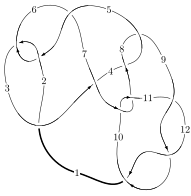
\includegraphics[width=112pt]{../../../GIT/diagram.site/Diagrams/png/2379_12n_0290.png}\\
\ \ \ A knot diagram\footnotemark}&
\allowdisplaybreaks
\textbf{Linearized knot diagam} \\
\cline{2-2}
 &
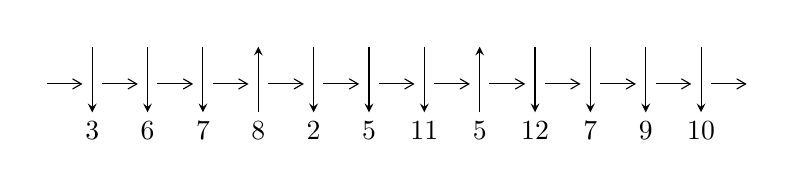
\begin{tikzpicture}[x=20pt, y=17pt]
	% nodes
	\node (C0) at (0, 0) {};
	\node (C1) at (1, 0) {};
	\node (C1U) at (1, +1) {};
	\node (C1D) at (1, -1) {3};

	\node (C2) at (2, 0) {};
	\node (C2U) at (2, +1) {};
	\node (C2D) at (2, -1) {6};

	\node (C3) at (3, 0) {};
	\node (C3U) at (3, +1) {};
	\node (C3D) at (3, -1) {7};

	\node (C4) at (4, 0) {};
	\node (C4U) at (4, +1) {};
	\node (C4D) at (4, -1) {8};

	\node (C5) at (5, 0) {};
	\node (C5U) at (5, +1) {};
	\node (C5D) at (5, -1) {2};

	\node (C6) at (6, 0) {};
	\node (C6U) at (6, +1) {};
	\node (C6D) at (6, -1) {5};

	\node (C7) at (7, 0) {};
	\node (C7U) at (7, +1) {};
	\node (C7D) at (7, -1) {11};

	\node (C8) at (8, 0) {};
	\node (C8U) at (8, +1) {};
	\node (C8D) at (8, -1) {5};

	\node (C9) at (9, 0) {};
	\node (C9U) at (9, +1) {};
	\node (C9D) at (9, -1) {12};

	\node (C10) at (10, 0) {};
	\node (C10U) at (10, +1) {};
	\node (C10D) at (10, -1) {7};

	\node (C11) at (11, 0) {};
	\node (C11U) at (11, +1) {};
	\node (C11D) at (11, -1) {9};

	\node (C12) at (12, 0) {};
	\node (C12U) at (12, +1) {};
	\node (C12D) at (12, -1) {10};
	\node (C13) at (13, 0) {};

	% arrows
	\draw[->,>={angle 60}]
	(C0) edge (C1) (C1) edge (C2) (C2) edge (C3) (C3) edge (C4) (C4) edge (C5) (C5) edge (C6) (C6) edge (C7) (C7) edge (C8) (C8) edge (C9) (C9) edge (C10) (C10) edge (C11) (C11) edge (C12) (C12) edge (C13) ;	\draw[->,>=stealth]
	(C1U) edge (C1D) (C2U) edge (C2D) (C3U) edge (C3D) (C4D) edge (C4U) (C5U) edge (C5D) (C6U) edge (C6D) (C7U) edge (C7D) (C8D) edge (C8U) (C9U) edge (C9D) (C10U) edge (C10D) (C11U) edge (C11D) (C12U) edge (C12D) ;
	\end{tikzpicture} \\
\hhline{~~} \\& 
\textbf{Solving Sequence} \\ \cline{2-2} 
 &
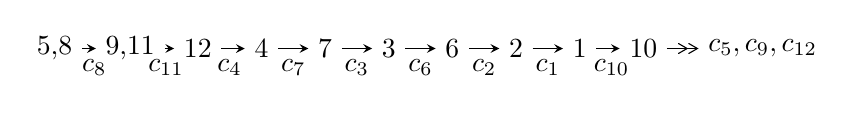
\begin{tikzpicture}[x=23pt, y=7pt]
	% node
	\node (A0) at (-1/8, 0) {5,8};
	\node (A1) at (17/16, 0) {9,11};
	\node (A2) at (17/8, 0) {12};
	\node (A3) at (25/8, 0) {4};
	\node (A4) at (33/8, 0) {7};
	\node (A5) at (41/8, 0) {3};
	\node (A6) at (49/8, 0) {6};
	\node (A7) at (57/8, 0) {2};
	\node (A8) at (65/8, 0) {1};
	\node (A9) at (73/8, 0) {10};
	\node (C1) at (1/2, -1) {$c_{8}$};
	\node (C2) at (13/8, -1) {$c_{11}$};
	\node (C3) at (21/8, -1) {$c_{4}$};
	\node (C4) at (29/8, -1) {$c_{7}$};
	\node (C5) at (37/8, -1) {$c_{3}$};
	\node (C6) at (45/8, -1) {$c_{6}$};
	\node (C7) at (53/8, -1) {$c_{2}$};
	\node (C8) at (61/8, -1) {$c_{1}$};
	\node (C9) at (69/8, -1) {$c_{10}$};
	\node (A10) at (11, 0) {$c_{5},c_{9},c_{12}$};

	% edge
	\draw[->,>=stealth]	
	(A0) edge (A1) (A1) edge (A2) (A2) edge (A3) (A3) edge (A4) (A4) edge (A5) (A5) edge (A6) (A6) edge (A7) (A7) edge (A8) (A8) edge (A9) ;
	\draw[->>,>={angle 60}]	
	(A9) edge (A10);
\end{tikzpicture} \\ 

\end{tabular} \\

\footnotetext{
The image of knot diagram is generated by the software ``\textbf{Draw programme}" developed by Andrew Bartholomew(\url{http://www.layer8.co.uk/maths/draw/index.htm\#Running-draw}), where we modified some parts for our purpose(\url{https://github.com/CATsTAILs/LinksPainter}).
}\phantom \\ \newline 
\centering \textbf{Ideals for irreducible components\footnotemark of $X_{\text{par}}$} 
 
\begin{align*}
I^u_{1}&=\langle 
-2.68465\times10^{94} u^{40}-9.84743\times10^{94} u^{39}+\cdots+1.38333\times10^{95} b-5.11987\times10^{96},\\
\phantom{I^u_{1}}&\phantom{= \langle  }-4.36327\times10^{94} u^{40}-1.61063\times10^{95} u^{39}+\cdots+2.76666\times10^{95} a-8.27022\times10^{96},\\
\phantom{I^u_{1}}&\phantom{= \langle  }u^{41}+4 u^{40}+\cdots+544 u+64\rangle \\
I^u_{2}&=\langle 
b,\;a-1,\;u+1\rangle \\
\\
I^v_{1}&=\langle 
a,\;26 v^5+33 v^4+317 v^3+123 v^2+413 b+89 v+685,\;v^6+3 v^5+15 v^4+24 v^3+11 v^2+6 v+1\rangle \\
\end{align*}
\raggedright * 3 irreducible components of $\dim_{\mathbb{C}}=0$, with total 48 representations.\\
\footnotetext{All coefficients of polynomials are rational numbers. But the coefficients are sometimes approximated in decimal forms when there is not enough margin.}
\newpage
\renewcommand{\arraystretch}{1}
\centering \section*{I. $I^u_{1}= \langle -2.68\times10^{94} u^{40}-9.85\times10^{94} u^{39}+\cdots+1.38\times10^{95} b-5.12\times10^{96},\;-4.36\times10^{94} u^{40}-1.61\times10^{95} u^{39}+\cdots+2.77\times10^{95} a-8.27\times10^{96},\;u^{41}+4 u^{40}+\cdots+544 u+64 \rangle$}
\flushleft \textbf{(i) Arc colorings}\\
\begin{tabular}{m{7pt} m{180pt} m{7pt} m{180pt} }
\flushright $a_{5}=$&$\begin{pmatrix}0\\u\end{pmatrix}$ \\
\flushright $a_{8}=$&$\begin{pmatrix}1\\0\end{pmatrix}$ \\
\flushright $a_{9}=$&$\begin{pmatrix}1\\- u^2\end{pmatrix}$ \\
\flushright $a_{11}=$&$\begin{pmatrix}0.157709 u^{40}+0.582157 u^{39}+\cdots+171.531 u+29.8924\\0.194072 u^{40}+0.711864 u^{39}+\cdots+205.306 u+37.0112\end{pmatrix}$ \\
\flushright $a_{12}=$&$\begin{pmatrix}-0.0560706 u^{40}-0.198690 u^{39}+\cdots-50.1633 u-10.2342\\0.220015 u^{40}+0.806259 u^{39}+\cdots+232.028 u+41.7645\end{pmatrix}$ \\
\flushright $a_{4}=$&$\begin{pmatrix}- u\\u\end{pmatrix}$ \\
\flushright $a_{7}=$&$\begin{pmatrix}-0.0860026 u^{40}-0.314486 u^{39}+\cdots-88.7056 u-16.8751\\0.244795 u^{40}+0.889941 u^{39}+\cdots+248.405 u+43.2805\end{pmatrix}$ \\
\flushright $a_{3}=$&$\begin{pmatrix}-0.0998198 u^{40}-0.360991 u^{39}+\cdots-89.6766 u-14.8006\\0.137856 u^{40}+0.501525 u^{39}+\cdots+141.893 u+24.7433\end{pmatrix}$ \\
\flushright $a_{6}=$&$\begin{pmatrix}-0.0860026 u^{40}-0.314486 u^{39}+\cdots-88.7056 u-16.8751\\0.253986 u^{40}+0.923580 u^{39}+\cdots+258.962 u+45.1700\end{pmatrix}$ \\
\flushright $a_{2}=$&$\begin{pmatrix}-0.214458 u^{40}-0.770687 u^{39}+\cdots-201.880 u-34.5510\\0.344343 u^{40}+1.25111 u^{39}+\cdots+349.391 u+60.8829\end{pmatrix}$ \\
\flushright $a_{1}=$&$\begin{pmatrix}-0.158792 u^{40}-0.575454 u^{39}+\cdots-159.700 u-26.4054\\0.269010 u^{40}+0.976627 u^{39}+\cdots+270.728 u+47.1022\end{pmatrix}$ \\
\flushright $a_{10}=$&$\begin{pmatrix}0.357088 u^{40}+1.31046 u^{39}+\cdots+376.594 u+66.5801\\-0.262269 u^{40}-0.954859 u^{39}+\cdots-266.063 u-46.3657\end{pmatrix}$\\&\end{tabular}
\flushleft \textbf{(ii) Obstruction class $= -1$}\\~\\
\flushleft \textbf{(iii) Cusp Shapes $= -2.16290 u^{40}-7.86224 u^{39}+\cdots-2195.29 u-401.897$}\\~\\
\newpage\renewcommand{\arraystretch}{1}
\flushleft \textbf{(iv) u-Polynomials at the component}\newline \\
\begin{tabular}{m{50pt}|m{274pt}}
Crossings & \hspace{64pt}u-Polynomials at each crossing \\
\hline $$\begin{aligned}c_{1},c_{6}\end{aligned}$$&$\begin{aligned}
&u^{41}+10 u^{40}+\cdots+124 u+1
\end{aligned}$\\
\hline $$\begin{aligned}c_{2},c_{5}\end{aligned}$$&$\begin{aligned}
&u^{41}+4 u^{40}+\cdots-8 u+1
\end{aligned}$\\
\hline $$\begin{aligned}c_{3}\end{aligned}$$&$\begin{aligned}
&u^{41}-2 u^{40}+\cdots-56802 u+4129
\end{aligned}$\\
\hline $$\begin{aligned}c_{4},c_{8}\end{aligned}$$&$\begin{aligned}
&u^{41}+4 u^{40}+\cdots+544 u+64
\end{aligned}$\\
\hline $$\begin{aligned}c_{7},c_{10}\end{aligned}$$&$\begin{aligned}
&u^{41}+4 u^{40}+\cdots-2 u+2
\end{aligned}$\\
\hline $$\begin{aligned}c_{9},c_{11},c_{12}\end{aligned}$$&$\begin{aligned}
&u^{41}-5 u^{40}+\cdots-11 u-1
\end{aligned}$\\
\hline
\end{tabular}\\~\\
\newpage\renewcommand{\arraystretch}{1}
\flushleft \textbf{(v) Riley Polynomials at the component}\newline \\
\begin{tabular}{m{50pt}|m{274pt}}
Crossings & \hspace{64pt}Riley Polynomials at each crossing \\
\hline $$\begin{aligned}c_{1},c_{6}\end{aligned}$$&$\begin{aligned}
&y^{41}+46 y^{40}+\cdots+12420 y-1
\end{aligned}$\\
\hline $$\begin{aligned}c_{2},c_{5}\end{aligned}$$&$\begin{aligned}
&y^{41}-10 y^{40}+\cdots+124 y-1
\end{aligned}$\\
\hline $$\begin{aligned}c_{3}\end{aligned}$$&$\begin{aligned}
&y^{41}+106 y^{40}+\cdots+3427830276 y-17048641
\end{aligned}$\\
\hline $$\begin{aligned}c_{4},c_{8}\end{aligned}$$&$\begin{aligned}
&y^{41}-36 y^{40}+\cdots+46080 y-4096
\end{aligned}$\\
\hline $$\begin{aligned}c_{7},c_{10}\end{aligned}$$&$\begin{aligned}
&y^{41}+42 y^{39}+\cdots+24 y-4
\end{aligned}$\\
\hline $$\begin{aligned}c_{9},c_{11},c_{12}\end{aligned}$$&$\begin{aligned}
&y^{41}-29 y^{40}+\cdots+141 y-1
\end{aligned}$\\
\hline
\end{tabular}\\~\\
\newpage\flushleft \textbf{(vi) Complex Volumes and Cusp Shapes}
$$\begin{array}{c|c|c}  
\text{Solutions to }I^u_{1}& \I (\text{vol} + \sqrt{-1}CS) & \text{Cusp shape}\\
 \hline 
\begin{aligned}
u &= \phantom{-}0.900371 + 0.275130 I \\
a &= -0.07966 - 1.47335 I \\
b &= \phantom{-}0.570501 + 0.849499 I\end{aligned}
 & -1.03538 + 3.10516 I & -9.19728 - 4.58914 I \\ \hline\begin{aligned}
u &= \phantom{-}0.900371 - 0.275130 I \\
a &= -0.07966 + 1.47335 I \\
b &= \phantom{-}0.570501 - 0.849499 I\end{aligned}
 & -1.03538 - 3.10516 I & -9.19728 + 4.58914 I \\ \hline\begin{aligned}
u &= -0.863117 + 0.163519 I \\
a &= \phantom{-}0.530392 - 1.038990 I \\
b &= \phantom{-}0.906841 + 0.441301 I\end{aligned}
 & -0.434343 - 0.606208 I & -8.36824 + 3.20718 I \\ \hline\begin{aligned}
u &= -0.863117 - 0.163519 I \\
a &= \phantom{-}0.530392 + 1.038990 I \\
b &= \phantom{-}0.906841 - 0.441301 I\end{aligned}
 & -0.434343 + 0.606208 I & -8.36824 - 3.20718 I \\ \hline\begin{aligned}
u &= -1.118190 + 0.134810 I \\
a &= \phantom{-}0.285482 + 1.154880 I \\
b &= -0.692354 - 0.679657 I\end{aligned}
 & \phantom{-}2.14754 - 4.46827 I & -5.46325 + 6.31020 I \\ \hline\begin{aligned}
u &= -1.118190 - 0.134810 I \\
a &= \phantom{-}0.285482 - 1.154880 I \\
b &= -0.692354 + 0.679657 I\end{aligned}
 & \phantom{-}2.14754 + 4.46827 I & -5.46325 - 6.31020 I \\ \hline\begin{aligned}
u &= -0.208887 + 0.817072 I \\
a &= \phantom{-}0.191298 - 0.000456 I \\
b &= -1.390780 + 0.124154 I\end{aligned}
 & -6.67711 + 2.45351 I & -15.2931 - 1.4222 I \\ \hline\begin{aligned}
u &= -0.208887 - 0.817072 I \\
a &= \phantom{-}0.191298 + 0.000456 I \\
b &= -1.390780 - 0.124154 I\end{aligned}
 & -6.67711 - 2.45351 I & -15.2931 + 1.4222 I \\ \hline\begin{aligned}
u &= -0.142298 + 0.686085 I \\
a &= \phantom{-}0.754137 - 0.156560 I \\
b &= \phantom{-}0.609820 - 0.257002 I\end{aligned}
 & -0.95163 + 1.08981 I & -8.28855 - 6.14268 I \\ \hline\begin{aligned}
u &= -0.142298 - 0.686085 I \\
a &= \phantom{-}0.754137 + 0.156560 I \\
b &= \phantom{-}0.609820 + 0.257002 I\end{aligned}
 & -0.95163 - 1.08981 I & -8.28855 + 6.14268 I\\
 \hline 
 \end{array}$$\newpage$$\begin{array}{c|c|c}  
\text{Solutions to }I^u_{1}& \I (\text{vol} + \sqrt{-1}CS) & \text{Cusp shape}\\
 \hline 
\begin{aligned}
u &= \phantom{-}1.320790 + 0.205247 I \\
a &= \phantom{-}0.272392 + 0.830191 I \\
b &= -0.359803 - 0.924561 I\end{aligned}
 & \phantom{-}3.58935 + 0.36497 I & \phantom{-0.000000 } 0 \\ \hline\begin{aligned}
u &= \phantom{-}1.320790 - 0.205247 I \\
a &= \phantom{-}0.272392 - 0.830191 I \\
b &= -0.359803 + 0.924561 I\end{aligned}
 & \phantom{-}3.58935 - 0.36497 I & \phantom{-0.000000 } 0 \\ \hline\begin{aligned}
u &= -1.47758 + 0.08314 I \\
a &= -0.028558 + 0.821385 I \\
b &= \phantom{-}1.27898 - 1.15594 I\end{aligned}
 & \phantom{-}7.32002 + 1.31400 I & \phantom{-0.000000 } 0 \\ \hline\begin{aligned}
u &= -1.47758 - 0.08314 I \\
a &= -0.028558 - 0.821385 I \\
b &= \phantom{-}1.27898 + 1.15594 I\end{aligned}
 & \phantom{-}7.32002 - 1.31400 I & \phantom{-0.000000 } 0 \\ \hline\begin{aligned}
u &= \phantom{-}1.47211 + 0.17758 I \\
a &= -0.081855 - 0.839711 I \\
b &= \phantom{-}1.19530 + 1.24551 I\end{aligned}
 & \phantom{-}7.22140 + 5.18811 I & \phantom{-0.000000 } 0 \\ \hline\begin{aligned}
u &= \phantom{-}1.47211 - 0.17758 I \\
a &= -0.081855 + 0.839711 I \\
b &= \phantom{-}1.19530 - 1.24551 I\end{aligned}
 & \phantom{-}7.22140 - 5.18811 I & \phantom{-0.000000 } 0 \\ \hline\begin{aligned}
u &= -0.493631\phantom{ +0.000000I} \\
a &= \phantom{-}1.54896\phantom{ +0.000000I} \\
b &= -0.291712\phantom{ +0.000000I}\end{aligned}
 & -1.40989\phantom{ +0.000000I} & -5.76550\phantom{ +0.000000I} \\ \hline\begin{aligned}
u &= \phantom{-}0.55563 + 1.40865 I \\
a &= \phantom{-}0.332513 + 0.052129 I \\
b &= -0.033282 - 0.910556 I\end{aligned}
 & \phantom{-}4.81513 + 1.29204 I & \phantom{-0.000000 } 0 \\ \hline\begin{aligned}
u &= \phantom{-}0.55563 - 1.40865 I \\
a &= \phantom{-}0.332513 - 0.052129 I \\
b &= -0.033282 + 0.910556 I\end{aligned}
 & \phantom{-}4.81513 - 1.29204 I & \phantom{-0.000000 } 0 \\ \hline\begin{aligned}
u &= \phantom{-}0.279316 + 0.386457 I \\
a &= -3.05813 - 4.36695 I \\
b &= -0.098053 + 0.379909 I\end{aligned}
 & -2.86863 - 0.30349 I & \phantom{-}1.29089 - 11.45256 I\\
 \hline 
 \end{array}$$\newpage$$\begin{array}{c|c|c}  
\text{Solutions to }I^u_{1}& \I (\text{vol} + \sqrt{-1}CS) & \text{Cusp shape}\\
 \hline 
\begin{aligned}
u &= \phantom{-}0.279316 - 0.386457 I \\
a &= -3.05813 + 4.36695 I \\
b &= -0.098053 - 0.379909 I\end{aligned}
 & -2.86863 + 0.30349 I & \phantom{-}1.29089 + 11.45256 I \\ \hline\begin{aligned}
u &= -0.012640 + 0.387805 I \\
a &= -8.88584 + 0.60443 I \\
b &= -0.500213 + 0.034819 I\end{aligned}
 & \phantom{-}1.80837 - 2.87388 I & -39.8656 + 3.3819 I \\ \hline\begin{aligned}
u &= -0.012640 - 0.387805 I \\
a &= -8.88584 - 0.60443 I \\
b &= -0.500213 - 0.034819 I\end{aligned}
 & \phantom{-}1.80837 + 2.87388 I & -39.8656 - 3.3819 I \\ \hline\begin{aligned}
u &= -0.64609 + 1.49909 I \\
a &= \phantom{-}0.280505 - 0.050822 I \\
b &= -0.227266 + 0.902339 I\end{aligned}
 & \phantom{-}4.34862 + 5.20839 I & \phantom{-0.000000 } 0 \\ \hline\begin{aligned}
u &= -0.64609 - 1.49909 I \\
a &= \phantom{-}0.280505 + 0.050822 I \\
b &= -0.227266 - 0.902339 I\end{aligned}
 & \phantom{-}4.34862 - 5.20839 I & \phantom{-0.000000 } 0 \\ \hline\begin{aligned}
u &= -0.353952\phantom{ +0.000000I} \\
a &= \phantom{-}0.190811\phantom{ +0.000000I} \\
b &= -1.66327\phantom{ +0.000000I}\end{aligned}
 & -9.84381\phantom{ +0.000000I} & \phantom{-}14.6310\phantom{ +0.000000I} \\ \hline\begin{aligned}
u &= -1.50019 + 0.69974 I \\
a &= -0.107163 - 0.866028 I \\
b &= \phantom{-}0.797327 + 0.867883 I\end{aligned}
 & -1.34409 - 8.57415 I & \phantom{-0.000000 } 0 \\ \hline\begin{aligned}
u &= -1.50019 - 0.69974 I \\
a &= -0.107163 + 0.866028 I \\
b &= \phantom{-}0.797327 - 0.867883 I\end{aligned}
 & -1.34409 + 8.57415 I & \phantom{-0.000000 } 0 \\ \hline\begin{aligned}
u &= -0.305001\phantom{ +0.000000I} \\
a &= \phantom{-}1.67143\phantom{ +0.000000I} \\
b &= \phantom{-}0.580690\phantom{ +0.000000I}\end{aligned}
 & -1.10346\phantom{ +0.000000I} & -8.70760\phantom{ +0.000000I} \\ \hline\begin{aligned}
u &= -1.63935 + 0.45660 I \\
a &= -0.069974 + 0.912206 I \\
b &= -1.19023 - 1.18604 I\end{aligned}
 & \phantom{-}11.66750 - 7.74036 I & \phantom{-0.000000 } 0\\
 \hline 
 \end{array}$$\newpage$$\begin{array}{c|c|c}  
\text{Solutions to }I^u_{1}& \I (\text{vol} + \sqrt{-1}CS) & \text{Cusp shape}\\
 \hline 
\begin{aligned}
u &= -1.63935 - 0.45660 I \\
a &= -0.069974 - 0.912206 I \\
b &= -1.19023 + 1.18604 I\end{aligned}
 & \phantom{-}11.66750 + 7.74036 I & \phantom{-0.000000 } 0 \\ \hline\begin{aligned}
u &= \phantom{-}1.56194 + 0.67841 I \\
a &= \phantom{-}0.009027 + 0.726408 I \\
b &= \phantom{-}0.492906 - 0.964772 I\end{aligned}
 & \phantom{-}1.69219 + 4.01190 I & \phantom{-0.000000 } 0 \\ \hline\begin{aligned}
u &= \phantom{-}1.56194 - 0.67841 I \\
a &= \phantom{-}0.009027 - 0.726408 I \\
b &= \phantom{-}0.492906 + 0.964772 I\end{aligned}
 & \phantom{-}1.69219 - 4.01190 I & \phantom{-0.000000 } 0 \\ \hline\begin{aligned}
u &= \phantom{-}1.67787 + 0.37565 I \\
a &= -0.035629 - 0.893097 I \\
b &= -1.10249 + 1.25882 I\end{aligned}
 & \phantom{-}11.97710 + 1.09300 I & \phantom{-0.000000 } 0 \\ \hline\begin{aligned}
u &= \phantom{-}1.67787 - 0.37565 I \\
a &= -0.035629 + 0.893097 I \\
b &= -1.10249 - 1.25882 I\end{aligned}
 & \phantom{-}11.97710 - 1.09300 I & \phantom{-0.000000 } 0 \\ \hline\begin{aligned}
u &= -1.49517 + 0.90641 I \\
a &= \phantom{-}0.139383 - 0.997291 I \\
b &= \phantom{-}1.11424 + 1.19188 I\end{aligned}
 & \phantom{-}7.3447 - 13.9917 I & \phantom{-0.000000 } 0 \\ \hline\begin{aligned}
u &= -1.49517 - 0.90641 I \\
a &= \phantom{-}0.139383 + 0.997291 I \\
b &= \phantom{-}1.11424 - 1.19188 I\end{aligned}
 & \phantom{-}7.3447 + 13.9917 I & \phantom{-0.000000 } 0 \\ \hline\begin{aligned}
u &= \phantom{-}1.54232 + 0.88599 I \\
a &= \phantom{-}0.131039 + 0.948244 I \\
b &= \phantom{-}1.03138 - 1.24212 I\end{aligned}
 & \phantom{-}8.03425 + 7.41571 I & \phantom{-0.000000 } 0 \\ \hline\begin{aligned}
u &= \phantom{-}1.54232 - 0.88599 I \\
a &= \phantom{-}0.131039 - 0.948244 I \\
b &= \phantom{-}1.03138 + 1.24212 I\end{aligned}
 & \phantom{-}8.03425 - 7.41571 I & \phantom{-0.000000 } 0 \\ \hline\begin{aligned}
u &= -1.63054 + 0.83010 I \\
a &= -0.034959 - 0.425949 I \\
b &= \phantom{-}0.284331 + 0.549059 I\end{aligned}
 & -3.12842 - 0.82148 I & \phantom{-0.000000 } 0\\
 \hline 
 \end{array}$$\newpage$$\begin{array}{c|c|c}  
\text{Solutions to }I^u_{1}& \I (\text{vol} + \sqrt{-1}CS) & \text{Cusp shape}\\
 \hline 
\begin{aligned}
u &= -1.63054 - 0.83010 I \\
a &= -0.034959 + 0.425949 I \\
b &= \phantom{-}0.284331 - 0.549059 I\end{aligned}
 & -3.12842 + 0.82148 I & \phantom{-0.000000 } 0\\
 \hline 
 \end{array}$$\newpage\newpage\renewcommand{\arraystretch}{1}
\centering \section*{II. $I^u_{2}= \langle b,\;a-1,\;u+1 \rangle$}
\flushleft \textbf{(i) Arc colorings}\\
\begin{tabular}{m{7pt} m{180pt} m{7pt} m{180pt} }
\flushright $a_{5}=$&$\begin{pmatrix}0\\-1\end{pmatrix}$ \\
\flushright $a_{8}=$&$\begin{pmatrix}1\\0\end{pmatrix}$ \\
\flushright $a_{9}=$&$\begin{pmatrix}1\\-1\end{pmatrix}$ \\
\flushright $a_{11}=$&$\begin{pmatrix}1\\0\end{pmatrix}$ \\
\flushright $a_{12}=$&$\begin{pmatrix}0\\1\end{pmatrix}$ \\
\flushright $a_{4}=$&$\begin{pmatrix}1\\-1\end{pmatrix}$ \\
\flushright $a_{7}=$&$\begin{pmatrix}1\\0\end{pmatrix}$ \\
\flushright $a_{3}=$&$\begin{pmatrix}0\\-1\end{pmatrix}$ \\
\flushright $a_{6}=$&$\begin{pmatrix}1\\-1\end{pmatrix}$ \\
\flushright $a_{2}=$&$\begin{pmatrix}-1\\0\end{pmatrix}$ \\
\flushright $a_{1}=$&$\begin{pmatrix}-1\\1\end{pmatrix}$ \\
\flushright $a_{10}=$&$\begin{pmatrix}1\\0\end{pmatrix}$\\&\end{tabular}
\flushleft \textbf{(ii) Obstruction class $= 1$}\\~\\
\flushleft \textbf{(iii) Cusp Shapes $= -12$}\\~\\
\newpage\renewcommand{\arraystretch}{1}
\flushleft \textbf{(iv) u-Polynomials at the component}\newline \\
\begin{tabular}{m{50pt}|m{274pt}}
Crossings & \hspace{64pt}u-Polynomials at each crossing \\
\hline $$\begin{aligned}c_{1},c_{2},c_{3}\\c_{4},c_{9}\end{aligned}$$&$\begin{aligned}
&u-1
\end{aligned}$\\
\hline $$\begin{aligned}c_{5},c_{6},c_{8}\\c_{11},c_{12}\end{aligned}$$&$\begin{aligned}
&u+1
\end{aligned}$\\
\hline $$\begin{aligned}c_{7},c_{10}\end{aligned}$$&$\begin{aligned}
&u
\end{aligned}$\\
\hline
\end{tabular}\\~\\
\newpage\renewcommand{\arraystretch}{1}
\flushleft \textbf{(v) Riley Polynomials at the component}\newline \\
\begin{tabular}{m{50pt}|m{274pt}}
Crossings & \hspace{64pt}Riley Polynomials at each crossing \\
\hline $$\begin{aligned}c_{1},c_{2},c_{3}\\c_{4},c_{5},c_{6}\\c_{8},c_{9},c_{11}\\c_{12}\end{aligned}$$&$\begin{aligned}
&y-1
\end{aligned}$\\
\hline $$\begin{aligned}c_{7},c_{10}\end{aligned}$$&$\begin{aligned}
&y
\end{aligned}$\\
\hline
\end{tabular}\\~\\
\newpage\flushleft \textbf{(vi) Complex Volumes and Cusp Shapes}
$$\begin{array}{c|c|c}  
\text{Solutions to }I^u_{2}& \I (\text{vol} + \sqrt{-1}CS) & \text{Cusp shape}\\
 \hline 
\begin{aligned}
u &= -1.00000\phantom{ +0.000000I} \\
a &= \phantom{-}1.00000\phantom{ +0.000000I} \\
b &= \phantom{-0.000000 } 0\end{aligned}
 & -3.28987\phantom{ +0.000000I} & -12.0000\phantom{ +0.000000I}\\
 \hline 
 \end{array}$$\newpage\newpage\renewcommand{\arraystretch}{1}
\centering \section*{III. $I^v_{1}= \langle a,\;26 v^5+33 v^4+\cdots+413 b+685,\;v^6+3 v^5+15 v^4+24 v^3+11 v^2+6 v+1 \rangle$}
\flushleft \textbf{(i) Arc colorings}\\
\begin{tabular}{m{7pt} m{180pt} m{7pt} m{180pt} }
\flushright $a_{5}=$&$\begin{pmatrix}v\\0\end{pmatrix}$ \\
\flushright $a_{8}=$&$\begin{pmatrix}1\\0\end{pmatrix}$ \\
\flushright $a_{9}=$&$\begin{pmatrix}1\\0\end{pmatrix}$ \\
\flushright $a_{11}=$&$\begin{pmatrix}0\\-0.0629540 v^{5}-0.0799031 v^{4}+\cdots-0.215496 v-1.65860\end{pmatrix}$ \\
\flushright $a_{12}=$&$\begin{pmatrix}0.0629540 v^{5}+0.0799031 v^{4}+\cdots+0.215496 v+1.65860\\-0.0629540 v^{5}-0.0799031 v^{4}+\cdots-0.215496 v-1.65860\end{pmatrix}$ \\
\flushright $a_{4}=$&$\begin{pmatrix}v\\0\end{pmatrix}$ \\
\flushright $a_{7}=$&$\begin{pmatrix}1\\-0.0629540 v^{5}-0.0799031 v^{4}+\cdots-0.215496 v-2.65860\end{pmatrix}$ \\
\flushright $a_{3}=$&$\begin{pmatrix}-0.108959 v^{5}-0.176755 v^{4}+\cdots+3.28087 v-0.0629540\\0.326877 v^{5}+0.530266 v^{4}+\cdots-5.84262 v+0.188862\end{pmatrix}$ \\
\flushright $a_{6}=$&$\begin{pmatrix}-0.150121 v^{5}-0.421308 v^{4}+\cdots-0.590799 v+0.891041\\-0.0629540 v^{5}-0.0799031 v^{4}+\cdots-0.215496 v-2.65860\end{pmatrix}$ \\
\flushright $a_{2}=$&$\begin{pmatrix}-0.600484 v^{5}-1.68523 v^{4}+\cdots-2.36320 v-1.43584\\1.26392 v^{5}+3.45036 v^{4}+\cdots+4.94189 v+3.53027\end{pmatrix}$ \\
\flushright $a_{1}=$&$\begin{pmatrix}-1\\0.0629540 v^{5}+0.0799031 v^{4}+\cdots+0.215496 v+2.65860\end{pmatrix}$ \\
\flushright $a_{10}=$&$\begin{pmatrix}-0.0629540 v^{5}-0.0799031 v^{4}+\cdots-0.215496 v-1.65860\\0.0629540 v^{5}+0.0799031 v^{4}+\cdots+0.215496 v+2.65860\end{pmatrix}$\\&\end{tabular}
\flushleft \textbf{(ii) Obstruction class $= 1$}\\~\\
\flushleft \textbf{(iii) Cusp Shapes $= -\frac{3042}{413} v^5-\frac{8817}{413} v^4-\frac{44523}{413} v^3-\frac{68494}{413} v^2-\frac{24042}{413} v-\frac{18195}{413}$}\\~\\
\newpage\renewcommand{\arraystretch}{1}
\flushleft \textbf{(iv) u-Polynomials at the component}\newline \\
\begin{tabular}{m{50pt}|m{274pt}}
Crossings & \hspace{64pt}u-Polynomials at each crossing \\
\hline $$\begin{aligned}c_{1},c_{3}\end{aligned}$$&$\begin{aligned}
&(u^3- u^2+2 u-1)^2
\end{aligned}$\\
\hline $$\begin{aligned}c_{2}\end{aligned}$$&$\begin{aligned}
&(u^3+u^2-1)^2
\end{aligned}$\\
\hline $$\begin{aligned}c_{4},c_{8}\end{aligned}$$&$\begin{aligned}
&u^6
\end{aligned}$\\
\hline $$\begin{aligned}c_{5}\end{aligned}$$&$\begin{aligned}
&(u^3- u^2+1)^2
\end{aligned}$\\
\hline $$\begin{aligned}c_{6}\end{aligned}$$&$\begin{aligned}
&(u^3+u^2+2 u+1)^2
\end{aligned}$\\
\hline $$\begin{aligned}c_{7},c_{9}\end{aligned}$$&$\begin{aligned}
&(u^2+u-1)^3
\end{aligned}$\\
\hline $$\begin{aligned}c_{10},c_{11},c_{12}\end{aligned}$$&$\begin{aligned}
&(u^2- u-1)^3
\end{aligned}$\\
\hline
\end{tabular}\\~\\
\newpage\renewcommand{\arraystretch}{1}
\flushleft \textbf{(v) Riley Polynomials at the component}\newline \\
\begin{tabular}{m{50pt}|m{274pt}}
Crossings & \hspace{64pt}Riley Polynomials at each crossing \\
\hline $$\begin{aligned}c_{1},c_{3},c_{6}\end{aligned}$$&$\begin{aligned}
&(y^3+3 y^2+2 y-1)^2
\end{aligned}$\\
\hline $$\begin{aligned}c_{2},c_{5}\end{aligned}$$&$\begin{aligned}
&(y^3- y^2+2 y-1)^2
\end{aligned}$\\
\hline $$\begin{aligned}c_{4},c_{8}\end{aligned}$$&$\begin{aligned}
&y^6
\end{aligned}$\\
\hline $$\begin{aligned}c_{7},c_{9},c_{10}\\c_{11},c_{12}\end{aligned}$$&$\begin{aligned}
&(y^2-3 y+1)^3
\end{aligned}$\\
\hline
\end{tabular}\\~\\
\newpage\flushleft \textbf{(vi) Complex Volumes and Cusp Shapes}
$$\begin{array}{c|c|c}  
\text{Solutions to }I^v_{1}& \I (\text{vol} + \sqrt{-1}CS) & \text{Cusp shape}\\
 \hline 
\begin{aligned}
v &= -1.49186\phantom{ +0.000000I} \\
a &= \phantom{-0.000000 } 0 \\
b &= \phantom{-}0.618034\phantom{ +0.000000I}\end{aligned}
 & -2.10041\phantom{ +0.000000I} & -19.6940\phantom{ +0.000000I} \\ \hline\begin{aligned}
v &= -0.082153 + 0.499284 I \\
a &= \phantom{-0.000000 } 0 \\
b &= -1.61803\phantom{ +0.000000I}\end{aligned}
 & -5.85852 + 2.82812 I & -6.54788 - 4.14885 I \\ \hline\begin{aligned}
v &= -0.082153 - 0.499284 I \\
a &= \phantom{-0.000000 } 0 \\
b &= -1.61803\phantom{ +0.000000I}\end{aligned}
 & -5.85852 - 2.82812 I & -6.54788 + 4.14885 I \\ \hline\begin{aligned}
v &= -0.217660\phantom{ +0.000000I} \\
a &= \phantom{-0.000000 } 0 \\
b &= -1.61803\phantom{ +0.000000I}\end{aligned}
 & -9.99610\phantom{ +0.000000I} & -38.1750\phantom{ +0.000000I} \\ \hline\begin{aligned}
v &= -0.56309 + 3.42214 I \\
a &= \phantom{-0.000000 } 0 \\
b &= \phantom{-}0.618034\phantom{ +0.000000I}\end{aligned}
 & \phantom{-}2.03717 + 2.82812 I & \phantom{-}0.982489 + 0.847836 I \\ \hline\begin{aligned}
v &= -0.56309 - 3.42214 I \\
a &= \phantom{-0.000000 } 0 \\
b &= \phantom{-}0.618034\phantom{ +0.000000I}\end{aligned}
 & \phantom{-}2.03717 - 2.82812 I & \phantom{-}0.982489 - 0.847836 I\\
 \hline 
 \end{array}$$\newpage
\newpage\renewcommand{\arraystretch}{1}
\centering \section*{ IV. u-Polynomials}
\begin{tabular}{m{50pt}|m{274pt}}
Crossings & \hspace{64pt}u-Polynomials at each crossing \\
\hline $$\begin{aligned}c_{1}\end{aligned}$$&$\begin{aligned}
&(u-1)(u^3- u^2+2 u-1)^2(u^{41}+10 u^{40}+\cdots+124 u+1)
\end{aligned}$\\
\hline $$\begin{aligned}c_{2}\end{aligned}$$&$\begin{aligned}
&(u-1)(u^3+u^2-1)^2(u^{41}+4 u^{40}+\cdots-8 u+1)
\end{aligned}$\\
\hline $$\begin{aligned}c_{3}\end{aligned}$$&$\begin{aligned}
&(u-1)(u^3- u^2+2 u-1)^2(u^{41}-2 u^{40}+\cdots-56802 u+4129)
\end{aligned}$\\
\hline $$\begin{aligned}c_{4}\end{aligned}$$&$\begin{aligned}
&u^6(u-1)(u^{41}+4 u^{40}+\cdots+544 u+64)
\end{aligned}$\\
\hline $$\begin{aligned}c_{5}\end{aligned}$$&$\begin{aligned}
&(u+1)(u^3- u^2+1)^2(u^{41}+4 u^{40}+\cdots-8 u+1)
\end{aligned}$\\
\hline $$\begin{aligned}c_{6}\end{aligned}$$&$\begin{aligned}
&(u+1)(u^3+u^2+2 u+1)^2(u^{41}+10 u^{40}+\cdots+124 u+1)
\end{aligned}$\\
\hline $$\begin{aligned}c_{7}\end{aligned}$$&$\begin{aligned}
&u(u^2+u-1)^3(u^{41}+4 u^{40}+\cdots-2 u+2)
\end{aligned}$\\
\hline $$\begin{aligned}c_{8}\end{aligned}$$&$\begin{aligned}
&u^6(u+1)(u^{41}+4 u^{40}+\cdots+544 u+64)
\end{aligned}$\\
\hline $$\begin{aligned}c_{9}\end{aligned}$$&$\begin{aligned}
&(u-1)(u^2+u-1)^3(u^{41}-5 u^{40}+\cdots-11 u-1)
\end{aligned}$\\
\hline $$\begin{aligned}c_{10}\end{aligned}$$&$\begin{aligned}
&u(u^2- u-1)^3(u^{41}+4 u^{40}+\cdots-2 u+2)
\end{aligned}$\\
\hline $$\begin{aligned}c_{11},c_{12}\end{aligned}$$&$\begin{aligned}
&(u+1)(u^2- u-1)^3(u^{41}-5 u^{40}+\cdots-11 u-1)
\end{aligned}$\\
\hline
\end{tabular}\newpage\renewcommand{\arraystretch}{1}
\centering \section*{ V. Riley Polynomials}
\begin{tabular}{m{50pt}|m{274pt}}
Crossings & \hspace{64pt}Riley Polynomials at each crossing \\
\hline $$\begin{aligned}c_{1},c_{6}\end{aligned}$$&$\begin{aligned}
&(y-1)(y^3+3 y^2+2 y-1)^2(y^{41}+46 y^{40}+\cdots+12420 y-1)
\end{aligned}$\\
\hline $$\begin{aligned}c_{2},c_{5}\end{aligned}$$&$\begin{aligned}
&(y-1)(y^3- y^2+2 y-1)^2(y^{41}-10 y^{40}+\cdots+124 y-1)
\end{aligned}$\\
\hline $$\begin{aligned}c_{3}\end{aligned}$$&$\begin{aligned}
&(y-1)(y^3+3 y^2+2 y-1)^2\\
&\cdot(y^{41}+106 y^{40}+\cdots+3427830276 y-17048641)
\end{aligned}$\\
\hline $$\begin{aligned}c_{4},c_{8}\end{aligned}$$&$\begin{aligned}
&y^6(y-1)(y^{41}-36 y^{40}+\cdots+46080 y-4096)
\end{aligned}$\\
\hline $$\begin{aligned}c_{7},c_{10}\end{aligned}$$&$\begin{aligned}
&y(y^2-3 y+1)^3(y^{41}+42 y^{39}+\cdots+24 y-4)
\end{aligned}$\\
\hline $$\begin{aligned}c_{9},c_{11},c_{12}\end{aligned}$$&$\begin{aligned}
&(y-1)(y^2-3 y+1)^3(y^{41}-29 y^{40}+\cdots+141 y-1)
\end{aligned}$\\
\hline
\end{tabular}
\vskip 2pc
\end{document}